\section{Nuværende omkostninger i sundhedssektoren}
Det er relevant at se på omkostningerne i sundhedssektorens primære og sekundære sektor ved brug af den nuværende målemetode. (RELEVANT IFT. HVAD?? JEG TROR DER MANGLER NOGET HER)

\subsection{Primær sektor} \label{sec:nuv_primaer}
\label{sec:primaer_sektor_omkostninger}
Den subjektive målemetode, der på nuværende tidspunkt benyttes af $27,7~\%$ af praktiserende læger, foregår ved spørgeskema under en konsultation, medfører udgifter i den primære sundhedssektor \citep{munck2007}. Afhængigt af antal konsultationer, som den enkelte kroniker har behov for, kan omkostningerne i forbindelse med konsultation ved udfyldelse af spørgeskemaer stige, mens udarbejdelse og udskrifter af spørgeskemaer vil have relativt lave omkostninger.
\citeauthor{munck2007} udarbejdede i 2007 en rapport om hypertension i almen praksis. Her blev $159$ kontaktpersoner i almen praksis spurgt: "Sætter I jeres hypertensionspatienter til kontrol med fast tidsinterval? Hvis ja, angiv det typiske interval" (MÅSKE MARKERE DETTE CITAT KURSIVT??). Her svarede $92,5~\%$, at de sætter deres patienter til kontrol med et fast tidsinterval, hvor den gennemsnitlige interval er udregnet til $3,9$ måneder \citep{munck2007}. 

Hvis det, jævnfør \citeauthor{kronborg2008}, antages at $1/5$ af den voksne danske befolkning har hypertension, vil dette svare til omkring $900.000$ danskere \citep{folketal2016}. Hvis $900.000$ danskere skal til lægekonsultation á $137,93$ kroner hver $3,9$. måned, vil dette svare til en årsomkostning for sundhedssektoren på omkring $380$ millioner kroner \citep{honorartabel2016}. 

Den samlede medicinudgift i den primære sundhedssektor i Danmark i $2014$ lå på $11,6$ milliarder kroner, og Danmarks Statistik påpeger i denne sammenhæng, at blodtrykssænkende medicin og hjertemedicin er nogle af de mest anvendte former for medicin i Danmark \citep{dst2016}. 

Ifølge en rapport udarbejdet af \citeauthor{apotekerforeningen2012} oplyses der, at de mest udleverede blodtrykssænkende lægemiddeler i år 2012, døgndosis (DDD) oplyses for hver, var amlodipin (139 DDD), furosemid (94 DDD), ramipril (92 DDD), bendroflumenthiazid og kalium (85 DDD), enalapril (80 DDD), samt losartan (73 DDD). Dette svarer til samlet $563$ millioner DDD i 2012 for disse blodtrykssænkende lægemidler for hele den danske befolkning \citep{apotekerforeningen2012}. DDD beskriver den anbefaldede dosis som patienterne skal have i forhold til prisen medicinen koster per dosis per dag. Hvis aktivitetsarmbånd som en non-farmakologisk  behandling implementeres i den almene praksis, vil der kunne spares på medicin DDD for patienter med hypertension, såfremt implementeringen påvirker patienternes helbred positivt. Ud over besparelser på DDD vil bivirkninger ved lægemidlerne også kunne reduceres, hvilket vil resultere i bedre livskvalitet for patienterne, samt et lettere behandlingsforløb. Eksempler på de hyppigste bivirkningerne ved de fleste af de nævnte lægemidler (ER DET HYPIGSTE BIVIRKNINGER VED DE NÆVNTE LÆGEMIDLER?? HVAD ER "DE FLESTE AF DE NÆVNTE") er ødemer, dehydrering, træthed, hovedpine og svimmelhed. Den bedste medicinering mod hypertension er individuel, hvorfor det ofte er nødvendigt at finde de lægepræparater, der er mest effektive for den enkelte patient, uden at der er for mange bivirkninger, hvilket besværligør og forlænger patienternes behandling.

\subsection{Sekundær sektor}
Den sekundære sektor påvirkes også af hypertension, da sygdommen er skyld i ambulante besøg og indlæggelser. I $2014$ var der $49.875$ ambulante besøg i den offentlige sekundære sektor for patienter med diagnosen blodtryksforhøjelse af enten kendt eller ukendt årsag, hvilket svarer til en stigning på $8,35~\%$ siden $2012$, hvilket kan ses på \autoref{fig:hyp_sekundaer} \citep{sundhedsdatastyrelsen2016}. 

\begin{figure}[H]
\centering
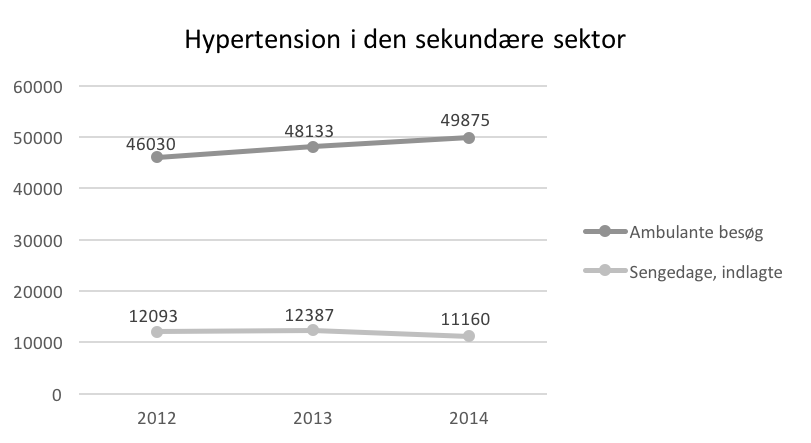
\includegraphics[width=0.8\textwidth]{figures/hyp_sekundaer}
\caption{Henvendelser i den offentlige sekundære sektor som følge af hypertension fra 2012 til 2014 \citep{sundhedsdatastyrelsen2016}.}
\label{fig:hyp_sekundaer}
\end{figure}

\noindent
Yderligere havde patienter med hypertension $11.160$ sengedage i forbindelse med indlæggelse på offentlige sygehuse i $2014$, hvilket var et fald i forholdt til de to foregående år \citep{sundhedsdatastyrelsen2016}. 

Jævnfør \citeauthor{takstvejledning2016} er taksten for et ambulant besøg  med journaloptagelse $1.421$ kroner uden nogen særlige procedurer, og taksten for en indlæggelse af en patient med hypertension er $12.597$ kroner indtil fire dage, der er det maksimale antal sengedage, der er dækket af denne takst. Ud over fire dage kan der opkræves en brugerbetaling for langliggertakst på $1.976$ kroner \citep{takstvejledning2016}. 

Hvis det antages, at ambulante besøg og antal sengedage i $2014$ er tilsvarende til henvendelser i år $2016$, så vil prisen for dette være omkring $210$ millioner kroner for ét år. 